\subsection{Use g2o to fit the curve}

In order to use g2o, we first abstract the curve fitting problem into a graph optimization. In this process, just remember that the \textbf{node is the optimization variable and the edge is the error term}. The graph optimization problem of curve fitting can be drawn as \autoref{fig:graph-fitting}.

\begin{figure}[!ht]
	\centering
	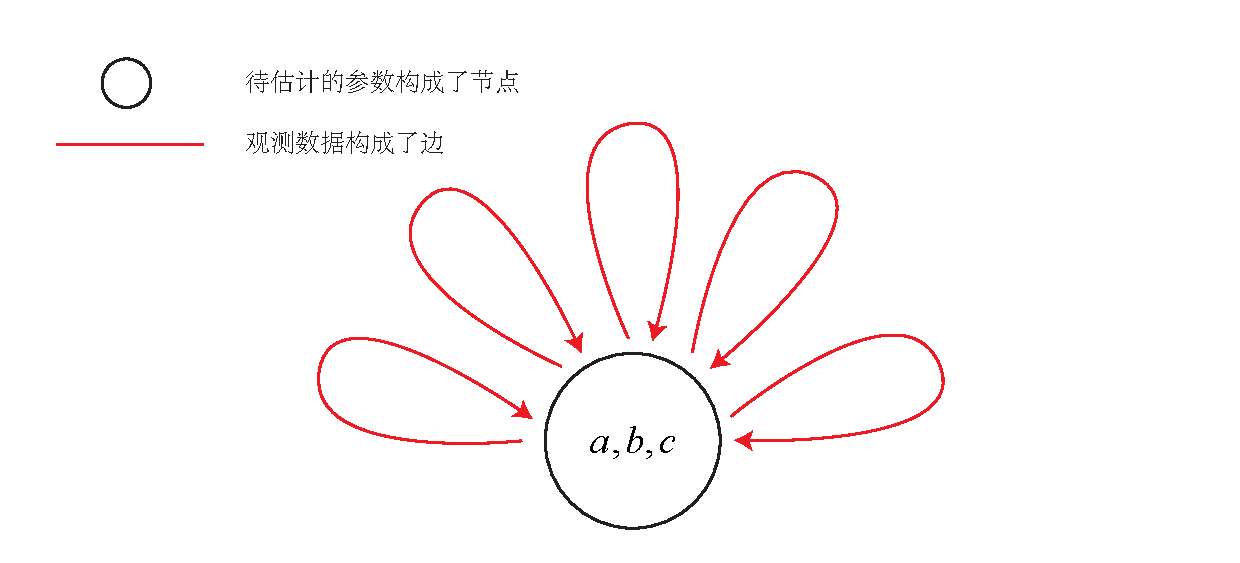
\includegraphics[width=.9 \textwidth]{chapter06/optimization/graphFitting.pdf}
	\caption{The curve is fitted to the corresponding graph optimization model. (There are some signs like Huawei.)}
	\label{fig:graph-fitting}
\end{figure}

In the curve fitting problem, the whole problem has only one vertex: the parameters of the curve model are $a, b, c$ and each noisy data point constitutes an error term, that is, the edge of the graph optimization.
But the edges here are not the same as the ones we usually think.
They are \textbf{Unary Edge}, ie \textbf{connects only one vertex} - because the whole graph has only one vertex.
So in \autoref{fig:graph-fitting}, we can only paint it as if we are connected to ourselves.
In fact, one edge of graph optimization can be connected to one, two or more vertices, which mainly reflects how many optimization variables each error is related to.
In a slightly mysterious way, we call it \textbf{Hyper Edge}, the whole picture is called \textbf{Hyper Graph} \footnote{ obviously I personally don't like some tricks. I am a naturalist. }.

After figuring out the graph model, the next step is to build the model in g2o for optimization. As a g2o user, what we have to do mainly consists of the following steps:

\begin{enumerate}
	\item defines the type of vertex and edge.
	\item build diagram.
	\item selects the optimization algorithm.
	\item calls g2o for optimization and returns the result.
\end{enumerate}

This part is very similar to Ceres, of course, the program will be written differently. Let's demonstrate the program below.

\begin{lstlisting}[language=c++,caption=slambook/ch6/g2oCurveFitting.cpp]
#include <iostream>
#include <g2o/core/g2o_core_api.h>
#include <g2o/core/base_vertex.h>
#include <g2o/core/base_unary_edge.h>
#include <g2o/core/block_solver.h>
#include <g2o/core/optimization_algorithm_levenberg.h>
#include <g2o/core/optimization_algorithm_gauss_newton.h>
#include <g2o/core/optimization_algorithm_dogleg.h>
#include <g2o/solvers/dense/linear_solver_dense.h>
#include <Eigen/Core>
#include <opencv2/core/core.hpp>
#include <cmath>
#include <chrono>

Using namespace std;

// Vertex of the curve model, template parameters: optimized variable dimensions and data types
Class CurveFittingVertex : public g2o::BaseVertex<3, Eigen::Vector3d> {
Public:
    EIGEN_MAKE_ALIGNED_OPERATOR_NEW
    
    // reset
    Virtual void setToOriginImpl() override {
        _estimate << 0, 0, 0;
    }
    
    // update
    Virtual void oplusImpl(const double *update) override {
        _estimate += Eigen::Vector3d(update);
    }
    
    // save and read: leave blank
    Virtual bool read(istream &in) {}
    Virtual bool write(ostream &out) const {}
};

// Error model template parameters: observation dimension, type, join vertex type
Class CurveFittingEdge : public g2o::BaseUnaryEdge<1, double, CurveFittingVertex> {
Public:
    EIGEN_MAKE_ALIGNED_OPERATOR_NEW
    
    CurveFittingEdge(double x) : BaseUnaryEdge(), _x(x) {}
    
    // Calculate the curve model error
    Virtual void computeError() override {
        Const CurveFittingVertex *v = static_cast<const CurveFittingVertex *> (_vertices[0]);
        Const Eigen::Vector3d abc = v->estimate();
        _error(0, 0) = _measurement - std::exp(abc(0, 0) * _x * _x + abc(1, 0) * _x + abc(2, 0));
    }
    
    // Calculate the Jacobian matrix
    Virtual void linearizeOplus() override {
        Const CurveFittingVertex *v = static_cast<const CurveFittingVertex *> (_vertices[0]);
        Const Eigen::Vector3d abc = v->estimate();
        Double y = exp(abc[0] * _x * _x + abc[1] * _x + abc[2]);
        _jacobianOplusXi[0] = -_x * _x * y;
        _jacobianOplusXi[1] = -_x * y;
        _jacobianOplusXi[2] = -y;
    }
    
    Virtual bool read(istream &in) {}
    Virtual bool write(ostream &out) const {}
Public:
    Double _x; // x value, y value is _measurement
};

Int main(int argc, char **argv) {
    / / Omit the data generation part of the code
    // Build graph optimization, first set g2o
    Typedef g2o::BlockSolver<g2o::BlockSolverTraits<3, 1>> BlockSolverType; // Each error term has an optimized variable dimension of 3 and an error value dimension of 1
    Typedef g2o::LinearSolverDense<BlockSolverType::PoseMatrixType> LinearSolverType; // Linear solver type
    
    // Gradient descent method, which can be selected from GN, LM, DogLeg
    Auto solver = new g2o::OptimizationAlgorithmGaussNewton(
        G2o::make_unique<BlockSolverType>(g2o::make_unique<LinearSolverType>()));
    G2o::SparseOptimizer optimizer; // graph model
    optimizer.setAlgorithm(solver); // Set the solver
    optimizer.setVerbose(true); // Turn on debug output
    
    // Add vertices to the graph
    CurveFittingVertex *v = new CurveFittingVertex();
    V->setEstimate(Eigen::Vector3d(ae, be, ce));
    V->setId(0);
    optimizer.addVertex(v);
    
    // Add a side to the picture
    For (int i = 0; i < N; i++) {
        CurveFittingEdge *edge = new CurveFittingEdge(x_data[i]);
        Edge->setId(i);
        Edge->setVertex(0, v); // Set the vertices of the connection
        Edge->setMeasurement(y_data[i]); // Observe the value
        Edge->setInformation(Eigen::Matrix<double, 1, 1>::Identity() * 1 / (w_sigma * w_sigma)); // Information matrix: the inverse of the covariance matrix
        optimizer.addEdge(edge);
    }
    
    // Perform optimization
    Cout << "start optimization" << endl;
    Chrono::steady_clock::time_point t1 = chrono::steady_clock::now();
    optimizer.initializeOptimization();
    Optimizer.optimize(10);
    Chrono::steady_clock::time_point t2 = chrono::steady_clock::now();
    Chrono::duration<double> time_used = chrono::duration_cast<chrono::duration<double>>(t2 - t1);
    Cout << "solve time cost = " << time_used.count() << " seconds. " << endl;
    
    // output optimized value
    Eigen::Vector3d abc_estimate = v->estimate();
    Cout << "estimated model: " << abc_estimate.transpose() << endl;
    
    Return 0;
}
\end{lstlisting}

In this program, we derive the graph-optimized vertices and edges for curve fitting from g2o: CurveFittingVertex and CurveFittingEdge, which essentially extends the way g2o is used. These two classes are derived from the BaseVertex and BaseUnaryEdge classes, respectively. In the derived class, we rewrote important virtual functions:

\begin{enumerate}
  \item Update function for vertex: oplusImpl. We know that the most important part of the optimization process is the calculation of the incremental $\Delta \bm{x}$, which handles $\bm{x}_{k+1} = \bm{x}_k + \Delta The process of \bm{x}$.

  Readers may think that this is not something worth mentioning, because it is just a simple addition. Why doesn't g2o help us? In the curve fitting process, since the optimization variable (curve parameter) itself is located in \textbf{vector space}, this update calculation is indeed a simple addition. However, when the optimization variable is not in the vector space, for example, $\bm{x}$ is the camera pose, it does not necessarily have an addition operation. At this point, you need to redefine the behavior of \textbf{incremental increments on existing estimates}. According to the explanation in Lecture 4, we may use left-multiply update or right-multiply update instead of direct addition.

  \item The reset function of the  vertex: setToOriginImpl. This is trivial, we can zero the estimate.

  \item The error calculation function of the edge: computeError. This function takes the current estimate of the vertex to which the edge is connected and compares it to its observations based on the curve model. This is consistent with the error model in the least squares problem.

  \item The Jacobian function of the side: linearizeOplus. In this function we calculate the Jacobian of each edge relative to the vertex.

  \item Save and read disk functions: read, write. Since we don't want to do read/write operations, leave it blank.
\end{enumerate}

After defining the vertices and edges, we declare a graph model in the main function, then add the vertices and edges to the graph model according to the generated noise data, and finally call the optimization function to optimize. G2o will give an optimized result:

\clearpage

\begin{lstlisting}[language=sh,caption=Terminal output:]
Start optimization
Iteration= 0 chi2= 376785.128234 time= 3.3299e-05 cumTime= 3.3299e-05 edges= 100 schur= 0
Iteration= 1 chi2= 35673.566018 time= 1.3789e-05 cumTime= 4.7088e-05 edges= 100 schur= 0
Iteration= 2 chi2= 2195.012304 time= 1.2323e-05 cumTime= 5.9411e-05 edges= 100 schur= 0
Iteration= 3 chi2= 174.853126 time= 1.3302e-05 cumTime= 7.2713e-05 edges= 100 schur= 0
Iteration= 4 chi2= 102.779695 time= 1.2424e-05 cumTime= 8.5137e-05 edges= 100 schur= 0
Iteration= 5 chi2= 101.937194 time= 1.2523e-05 cumTime= 9.766e-05 edges= 100 schur= 0
Iteration= 6 chi2= 101.937020 time= 1.2268e-05 cumTime= 0.000109928 edges= 100 schur= 0
Iteration= 7 chi2= 101.937020 time= 1.2612e-05 cumTime= 0.00012254 edges= 100 schur= 0
Iteration= 8 chi2= 101.937020 time= 1.2159e-05 cumTime= 0.000134699 edges= 100 schur= 0
Iteration= 9 chi2= 101.937020 time= 1.2688e-05 cumTime= 0.000147387 edges= 100 schur= 0
Solve time cost = 0.000919301 seconds. 
Estimated model: 0.890912 2.1719 0.943629
\end{lstlisting}

We use the Gauss-Newton method for gradient descent, and after 9 iterations, we get the optimization results, which is similar to Ceres and handwritten Gauss-Newton method. From the perspective of running speed, our experimental conclusion is that handwriting is faster than g2o, and g2o is faster than Ceres. This is a generally intuitive experience, and versatility and efficiency are often contradictory. However, Ceres used automatic derivation in this experiment, and the solver configuration is not exactly the same as Gauss Newton, so it looks slower.
